\section{Постановка задачи} \label{p21}
\paragraph{}
Рассмотрим математическую модель двухзвенного манипулятора. Манипулятор состоит из неподвижного основания и двух абсолютно жестких звеньев $G_1, G_2$. Элементы конструкции соединены между собой двумя идеальными цилиндрическими шарнирами $O_1,$ и $O_2$ таким образом, что оба звена могут совершать движения только в горизонтальной или вертикальной плоскости. Центр масс $C_1$ звена $G_1$ лежит на луче $O_1 O_2.$ Положение центра масс $C_2$ звена $G_2$ не совпадает с положением шарнира $O_2$.

 \begin{figure}[h]
 	\centering
 	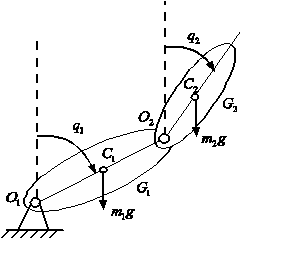
\includegraphics{manipulator}
 	\caption{Модель двузвенного манипулятора}
 	\label{fig:manip1}
 \end{figure}

Введем обозначения: $q_i (i=1, 2)$ --- углы поворотов звеньев манипулятора, показанные на рисунке; $l_i$ --- длина отрезка $O_i C_i;$ $l$ --- длина отрезка $O_1 O_2;$ $m_i$  ---  масса   $i$-го звена;   $I_i$ --- момент инерции  $i$-го звена относительно оси шарнира $O_i;$ $g$ --- ускорение свободного падения.

Выражение для кинетической энергии манипулятора имеет в таком случае следующий вид:
\begin{equation}
T = \frac12 ((I_1 + I_2 + m_2 l^2 + 2 m_2 l l_2 \cos q_2) \dot q_1^2 + (I_2 + m_2 l l_2 \cos q_2) \dot q_1 \dot q_2 + I_2 \dot q_2^2)
\end{equation}

Составим уравнения Лагранжа второго рода:

\begin{equation}
\begin{cases}
\displaystyle \frac{d}{dt} (\frac{\partial T}{\partial \dot q_1}) - \frac{\partial T}{\partial q_1} = M_1 + U_1, \\
\displaystyle \frac{d}{dt} (\frac{\partial T}{\partial \dot q_2}) - \frac{\partial T}{\partial q_2} = M_2 + U_2,
\end{cases}
\end{equation}

где $M_i$ --- момент, создаваемый силой тяжести в $i$-м шарнире. В случае манипулятора, совершающего движения в вертикальной плоскости, 
$$
\begin{array}{l}
M_1 = (m_1 l_1 + m_2 l) g \cos q_1, \\
M_2 = m_2 l_2 g \cos (q_1 + q_2),
\end{array}
$$
$U_i$ --- управление.

Из выражения для кинетической энергии $T$ находим уравнения движения

\begin{equation}
\begin{array}{l}
a_{11} \ddot q_1 + a_{12} \ddot q_2 - 2 m_2 l l_2 \sin q_2 \dot q_1 \dot q_2 - m_2 l l_2 \sin q_2 \dot q_2^2 = U_1,\\ 
a_{12} \ddot q_1 + a_{22} \ddot q_2 + m_2 l l_2 \sin q_2 \dot q_1^2 = U_2,\\
a_{11} (q_2) = m_2 l_1^2 + I_1 + I_2 + 2 m_2 l l_2 \cos q_2,\\
a_{12} (q_2)= I_2 + m_2 l l_2 \cos q_2, a_{22} = I_2
\end{array}
\end{equation}

\begin{equation}
\begin{array}{l}
	a_{11} \ddot q_1 + a_{12} \ddot q_2 - 2 m_2 l l_2 \sin q_2 \dot q_1 \dot q_2 - m_2 l l_2 \sin q_2 \dot q_2^2 = U_1,\\ 
	a_{12} \ddot q_1 + a_{22} \ddot q_2 + m_2 l l_2 \sin q_2 \dot q_1^2 = U_2,\\
	\dot x_1 = \sin(q_1(t)) - k * x_1(t), \\ 
	\dot x_2 = \sin(q_2(t)) - k * x_2(t), \\ 
	a_{11} (q_2) = m_2 l_1^2 + I_1 + I_2 + 2 m_2 l l_2 \cos q_2,\\
	a_{12} (q_2)= I_2 + m_2 l l_2 \cos q_2,\\ 
	a_{22} = I_2
\end{array}
\end{equation}

$U1 = -\mu_1 \sin(q_1(t)) - \frac{L}{k} \sin(q_1(t)) \cos(q_1(t)) (1 - e^{- k t}) + L x_1(t) \cos(q_1(t))$

$U2 = -\mu_2 \sin(q_2(t)) - \frac{L}{k} \sin(q_2(t)) \cos(q_2(t)) (1 - e^{- k t}) + L x_2(t) \cos(q_2(t))$

$q_1(0) = 0.5, \ \dot q_1(0) = -0.5, \ q_2(0) = 2.1, \ \dot q_2(0) = 0.3, \ x_1(0) = 0, \ x_2(0) = 0$

$$ I_1 = 3.33, \ I_2 = 3.33,  l = 1,  l_2 = 0.5,  m_2 = 10, \mu_1 = 5,  \mu_2 = 5, L = 1,  k = 1$$

Пусть $q=q(q_1, q_2)^{'}$ --– вектор обобщенных координат рассматриваемой механической системы и 
$$X = \{(q^0(t), \dot q^0(t)) : [t_0, + \infty) \to R^4, \left|q^0(t)\right| \le g_0, \left|\dot q^0(t) \right| \le g_1, \left|\ddot q^0(t)\right| \le g_2 \}$$

есть заданное множество программных движений манипулятора в виде ограниченных дважды непрерывно дифференцируемых функций $q=q^0(t)$ с ограниченными производными при $t \in [t_0, + \infty).$ Символом $\left| \cdot \right|$   обозначена евклидова норма вектора.

Пусть $(q^0(t), \dot q^0(t)) \in X$ --- какое-либо программное движение, реализуемое программным управлением $U = U^0(t).$ Таким образом, для обеспечения такого движения имеет место следующее управление
$$
\begin{array}{l}
U_1^0 (t) = a_{11} (q_2^0 (t)) \ddot q_1^0 (t) + a_{12} (q_2^0 (t)) \ddot q_2^0 (t) - 2 m_2 l l_2 \sin q_2^0 (t) \dot q_1^0 (t) \dot q_2^0 (t) - \\ 
- m_2 l l_2 \sin q_2^0 (t) - M_1^0 (t) \\
U_2^0 (t) = a_{12}^0 (t) \ddot q_1^0 (t) + I_2 \ddot q_2^0 (t) - M_2^0 (t) \\
\end{array}
$$
где $$M_1^0(t) = M_2^0(t) = 0$$ для случая манипулятора в горизонтальной плоскости
\begin{equation}
\begin{array}{l}
M_1^0 (t) = (m_1 l_1 + m_2 l) g \cos q_1^0 (t), \\
M_2^0 (t) = m_2 l_2 g \cos (q_1^0 (t) + q_2^0 (t))
\end{array}
\end{equation}

в случае манипулятора, функционирующего в вертикальной плоскости.

Введем возмущения $x_k = q_k - q_k^0(t), \quad \dot x_k = \dot q_k - \dot q_k^0(t), \quad k = 1, 2$

Составим уравнения возмущенного движения в векторно-матричном виде:
\begin{equation}
A^{(1)}(t, x) \ddot x = {\dot x^{'} C^{(1)}(t, x) \dot x} + Q^{(1)}(t,x) + Q^{(2)}(t, x, \dot x) + U^{(1)}, \label{2.2'}
\end{equation}

$$A^{(1)}(t, x) =
\begin{pmatrix}
a_{11} (q_2^0 (t) + x_2) && a_{12} (q_2^0 (t) + x_2) \\
a_{12} (q_2^0 (t) + x_2) && I_2 \\
\end{pmatrix}$$

$$Q^{(1)}(t,x)=F(t,x)p(x), \quad Q^{(2)}(t,x,\dot x)=D(t,x)\dot x, $$

$$C_1^{(1)}(t, x) = m_2 l l_2 \sin (q_2^0 (t) + x_2)
\begin{pmatrix}
0 && 1\\
1 && 1\\
\end{pmatrix}$$

$$C_2^{(1)}(t, x) = - m_2 l l_2 \sin (q_2^0 (t) + x_2)
\begin{pmatrix}
1 && 0\\
0 && 0\\
\end{pmatrix}$$

$$F(t, x) =
\begin{pmatrix}
f_{11}(t,x) && f_{12}(t,x) \\
f_{21}(t,x) && f_{22}(t,x)\\
\end{pmatrix},$$

$$p(x) =
\begin{pmatrix}
\sin(x_1/2) \\
\sin(x_2/2)\\
\end{pmatrix},$$

$$D(t, x) =
\begin{pmatrix}
d_{11} (t, x) && d_{12} (t, x) \\
d_{21} (t, x) && d_{22} (t, x) \\
\end{pmatrix},$$

$f_{11}(t,x) = 0 \{ + (- 2 m_1 l_1 - 2 m_2 l) g \sin (q_1^0 (t) + x_1 / 2) \}$

$f_{12}(t,x) = 4 m_2 g l l_2 \ddot q_1^0 (t) \sin (q_2^0 (t) + x_2 / 2) + 2 m_2 l l_2 \ddot q_2^0 (t) * \\ 
* \sin (q_2^0 (t) + x_2 / 2) + 4 m_2 l l_2 \cos (q_2(t) + x_2 / 2) \dot q_1^0 (t) \dot q_2^0 (t) + \\ 
+ 2 m_2 l l_2 \cos (q_2^0 (t) + x_2 / 2) (\dot q_2^0)^2$

$f_{21}(t,x) = 0 \{ + (-4 m_2 l_2 g \sin (q_1^0 (t) + q_2^0 (t) + x_1 /2 + x_2 / 2 \cos x_2 / 2)) \}$

$f_{22}(t,x) = 2 m_2 l l_2 \ddot q_2^0 (t) \sin (q_2^0 (t) + x_2 / 2) + 2 m_2 l l_2 \cos (q_2^0 (t) + x_2 /2) * \\ 
* (q_1^0 (t))^2 \{ + (-4 m_2 l_2 \sin (q_1^0 (t) + q_2^0 (t) + x_1 / 2 + x_2 /2) \cos x_1 /2) \}$

$$
\begin{array}{l}
d_{11}(t, x) = 2 m_2 l l_2 \sin(q_2^0 (t + x_1) \dot q_2^0 (t)) \\
d_{12}(t, x) = 2 m_2 l l_2 \sin(q_2^0 (t + x_1) \dot q_1^0 (t)) + 2 m_2 l l_2 \sin(q_1^0 (t) + x_2) \dot q_2^0 (t) \\
d_{21}(t, x) = - 2 m_2 l l_2 \sin (q_2^0 (t) + x_2) \dot q_1^0 (t) \\
d_{22}(t, x) = 0
\end{array}
$$

где слагаемые, заключенные в фигурные скобки, добавляются в случае вертикального манипулятора.

$$ U^{(1)} = U - U^{0}(t) $$

В главе рассматривается задача построения управляющего воздействия $$ U^{(1)} = U^{(1)}(t, x, \dot x), \quad U^{(1)} (t, 0, 0) \equiv 0 $$, при котором бы невозмущенное движение $\dot x = x = 0$  системы (2.2) было бы равномерно асимптотически устойчиво, или, иными словами, управление $$U = U^0(t) + U^{(1)}(t, q-q^0(t), \dot q - \dot q^0(t))$$

обеспечивало бы стабилизацию программного движения $(q^0(t), \dot q^0(t)) \in X$  системы (2.1).